\documentclass[a4paper]{article} 
\usepackage[14pt]{extsizes} % для того чтобы задать нестандартный 14-ый размер шрифта 
\usepackage[utf8]{inputenc} 
\usepackage[russian]{babel} 
\usepackage{amsmath,amsfonts,amssymb,amsthm,mathtools} 
\usepackage[left=20mm, top=15mm, right=15mm, bottom=15mm, nohead, footskip=10mm]{geometry} % настройки полей документа 

\begin{document} % начало документа 
% НАЧАЛО ТИТУЛЬНОГО ЛИСТА 
\begin{center} 
\hfill \break 
\large{Санкт-Петербургский Политехнический университет имени Петра Великого}\\ 
 
 \hfill \break 
\hfill\break 
\hfill \break 
\hfill \break 
\hfill \break 
\begin{center}\large{Отчёт по лабораторной работе №2} \end{center}  
\hfill \break 
\large{Тема: Численное интегрирование } 
\hfill \break 
\hfill \break 
 
\hfill \break 
\hfill \break 
\\ 
\hfill \break 
\hfill \break 
\end{center} 


\normalsize{ 
\begin{tabular}{cccc} 
Студент & : & Алексеева Мария Сергеевна\\\\ 
Группа & : & 5030103/00003 \\\\ 
Преподаватель & : & Козлов Константин Николаевич \\\\ 
\end{tabular} 
}\\ 
\hfill \break 
\hfill \break 
\hfill \break 
\begin{center} Санкт-Петербург 2022 \end{center} 
\thispagestyle{empty} % выключаем отображение номера для этой страницы 
 
% КОНЕЦ ТИТУЛЬНОГО ЛИСТА 
\newpage 
	
\section{Формулировка задачи и её формализация} 
Задача: Вычислить значение интеграла функции $y = x^4-6.2x^3+3.5x^2-7x-2.1$ c помощью квадратурной формулы "трех восьмых". Исследовать для данного метода зависимость погрешности от измельчения шага, сравнить теоретическую и фактическую погрешности и исследовать влияние заданной точности на количество вычислений.
\section{Алгоритм метода и условия его применимости} 
\subsection{Алгоритм}
Для того, чтобы вычислить определенный интеграл с помощью метода $3/8$ необходимо задать границы интегрирования, т.е. интервал $[a,b]$. В данном методе количество узлов n=4, а шаг между ними задается формулой $h=\dfrac{b-a}{3}$. Построив узлы $x_1...x_4$ по формуле $x_k=a+(k-1)*h$, вычислим значение интеграла:\\
 $ \int\limits_a^b f(x)dx= \dfrac{3h}{8}(f(a)+3f(a+2h)+3f(a+3h)+f(b))$.

\subsection{Условия применимости}
Интегрируемая функция должна быть непрерывной
 
\section{Предварительный анализ задачи} 
Для построения интеграла берется непрерывная функция => можно ожидать точного вычисления интеграла. Ожидается, что в первом исследование погрешность будет уменьшаться с увеличением количества точек, во втором фактическая погрешность должна быть меньше теоретической, в третьем при высокой точности необходимо большое количество вычислений.
\section{Тестовый пример с расчётами} 
В качестве примера рассмотрит простую функцию y = x на интервале [0;1].\\
1) $h = \dfrac{1-0}{3}=\dfrac{1}{3}$ \\
2) $x_1 = 0    x_2 =\dfrac{1}{3} x_3 =\dfrac{2}{3} x_4 = 1  $\\
3) $ \int\limits_0^1 xdx = \dfrac{3 \dfrac{1}{3}}{8}(0+3*\dfrac{1}{3}+3*\dfrac{2}{3}+1) = \dfrac{1}{8}*4=\dfrac{1}{2}$\\
4) $ \int\limits_0^1 xdx  = \dfrac{x^2}{2} |^{1} _{0}=\dfrac{1}{2}$\\
Видим, что значения при аналитическом и численном вычислении интеграла совпали.

 
\section{Подготовка контрольных тестов для иллюстрации метода} 

Интегрирование будет проводиться на отрезке [-1;1]. В качестве первого исследования будем дробить заданный интервал на более мелкие разибения и рассматривать погрешность в каждом случае. Для лучшего отслеживания зависимости кол-во точек в интервале каждый раз будет увеличиваться в два раза. Функция будет принимать интервал [a,b] и количество точек в нем, по эти данным будет строиться массив "разибения" с помощью linspace. С помощью цикла пройдемся по всем "мини-интервалам" , образовавшимся внутри [a,b] и для каждого будем считать значение интеграла, а затем суммировать.  Далее будет проведено исследование для сравнения точностей. Здесь будет использоваться правило Рунге: $\dfrac{|I_{2n}-I_n|}{15}<\epsilon$. Т.е. будут рассматриваться погрешности для разибений, который отличаются друг от друга по количеству точек в два раза. Найдя фактическую точность сравним ее с теоретической. Последнее исследование покажет как мелко нужно разбивать интервал для получения заданной точности.
  
\newpage
\section{Модульная структура программы} 
 
\begin{figure}[h!]
\begin{center}
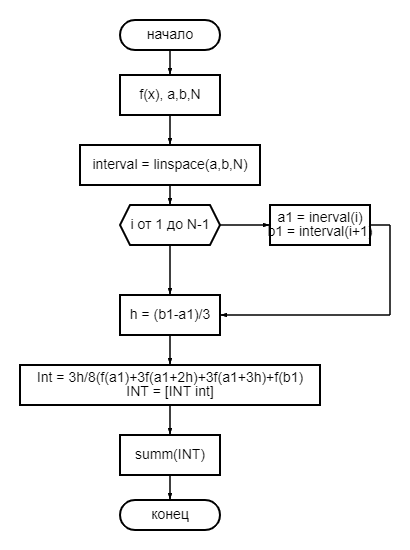
\includegraphics[scale=0.7]{схема с разбиением.png} 
\end{center}
\caption{Блок-схема метода 3/8 с учетом разбиения отрезка} \label{Рис1}
\end{figure}

\newpage
\section{Численный анализ решения задачи}


\subsection{Исследование зависимости погрешности от разбиения} 

\begin{figure}[h!]
\begin{center}
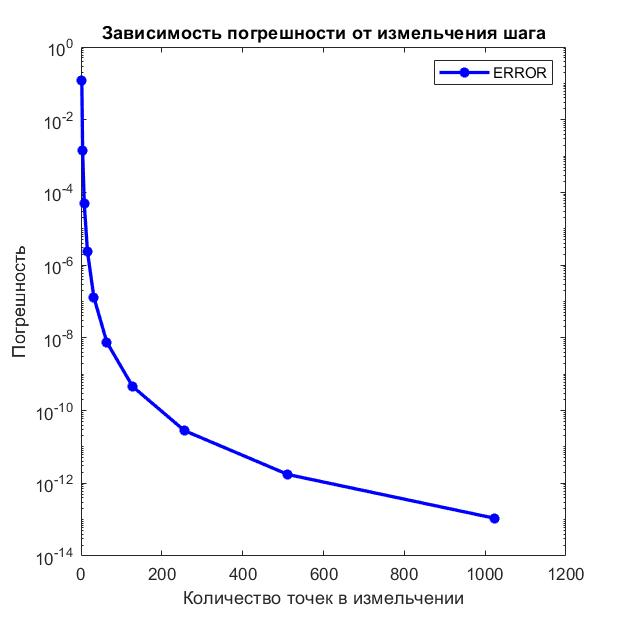
\includegraphics[scale=0.7]{погрешность от зимельчения шага.jpg} 
\end{center}
\caption{Зависимость погрешности от измельчения шага} \label{Рис2}
\end{figure}
На рисунке \ref{Рис2} мы наблюдаем, что при увеличении измельчения исходного интервала погрешность уменьшается, что и ожидалось.


\subsection{Сравнение теоретической и фактической точности} 

\begin{figure}[h!]
\begin{center}
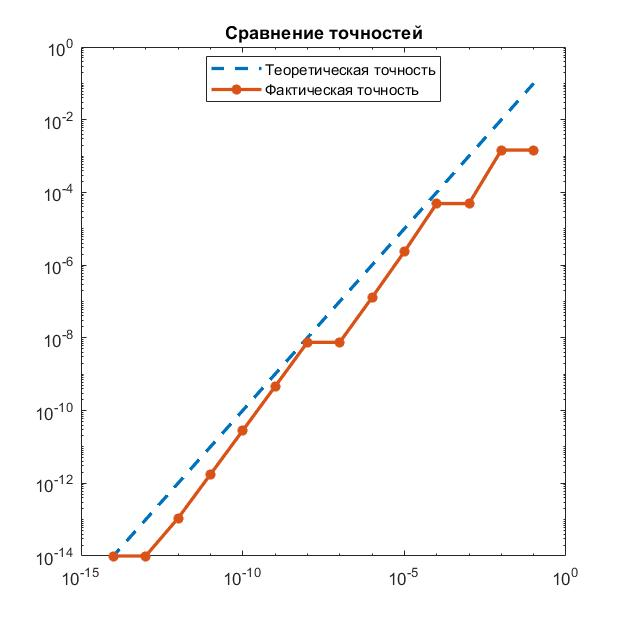
\includegraphics[scale=0.7]{сравнение точностей.jpg} 
\end{center}
\caption{Сравнение теоретической и фактической точности} \label{Рис3}
\end{figure}
На рисунке \ref{Рис3} c радостью можно отметить, что фактическая точность не превышает теоретической, что и ожидалось.\\

\subsection{Исследование влияния заданной точности на количество вычислений}
\begin{figure}[h!]
\begin{center}
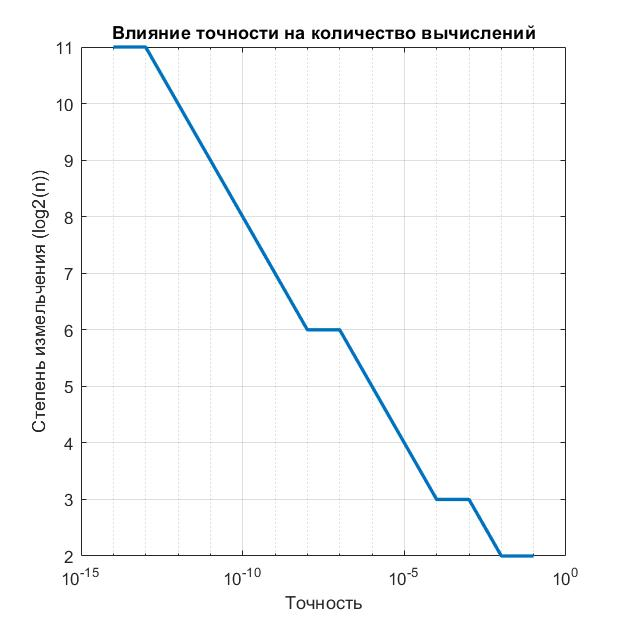
\includegraphics[scale=0.7]{влияние точности на кол-во вычислений.jpg} 
\end{center}
\caption{Исследование влияния заданной точности на количество вычислений} \label{Рис4}
\end{figure}


\begin{figure}[h!]
\begin{center}
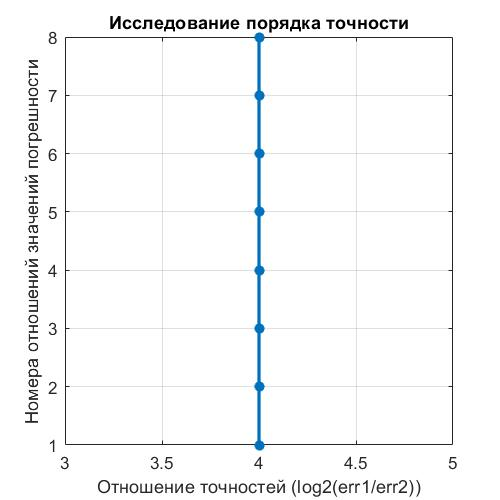
\includegraphics[scale=0.8]{порядок точности.jpg} 
\end{center}
\caption{Исследование влияния заданной точности на количество вычислений} \label{Рис5}
\end{figure}

 На рисунке \ref{Рис4}  изображен график, по оси икс на котором отмечается точность, по оси игрек - степень измельчения, то есть не количество точек, а степень двойки, т.к. ислледования проводились для постоянно увеличивающегося в два раза разбиения. Из исследования видно, что для лучше точности требуется большее количество разбиений отрезка.\\ 
На рисунке \ref{Рис5} изображени график, на котором мы видим значение алгебраического порядка точности. Для метода 3/8 этот порядок равен 4. Как видно из графика исследования порядок точности фактический совпадает с теоретическим. \\
\\
\\




\newpage 
\newpage
\section{Краткие выводы} 

\begin{itemize}
  \item Метод 3/8 позволяет вычислить интеграл с достаточно высокой точностью, если правильно подобрать разбиение отрезка.
  \item Все исследования удовлетворили предварительному анализу.
  \item Исследования показали, что для того, чтобы вычислять интеграл с минимальной погрешностью необходимо брать как можно большее разбиение. 
  \end{itemize}


\end{document} % КОНЕЦ ДОКУМЕНТА !

